\section{User Evaluation}
\subsection{Description}

\subsubsection{Introduction and hypotheses}
The user interface has been designed to look similar to current forum-style "social media". This choice of design was made such that the average user would be facing as little a hurdle as possible, in transitioning from their current forum of choice to this product. To test if this is actually the case the following \textit{null hypothesis} is posed:\newline
\textit{ - When presented with a product with similar features, but better security, users will not leave their current daily driver}

\subsubsection{Subjects}
The test subjects in the experiment were found at the university, in or close to our own hall. This means that the subjects in the test were all of rather similar educational programs. This would tend to cause the test subjects to be somewhat similar to our selves in mindset. The test subjects are also probably of a higher than average technical skill level and might be more familiar with forums than the average user.

\subsubsection{Materials}
The prototype is run as a simple interactive website controlled from a browser on a computer. The users use the computer's keyboard and mouse to navigate the prototype. As the prototype is programmed only using HTML, CSS and JavaScript there is no need for extra software other than the web browser.

\subsubsection{Methods and procedure}
\label{procedure}
The experiment is run in two stages: The first stage is using the qualitative method "think aloud", where the user is asked some questions while navigating the prototype. These questions are asked on the fly. The second stage is using the quantitative method "System Usability Scale (SUS)", which is an acknowledged questionnaire, that measures how the usability of the system was. Through these two methods the results can be triangulated to provide more certainty in the experiment.

\begin{figure}[H]
    \centering
    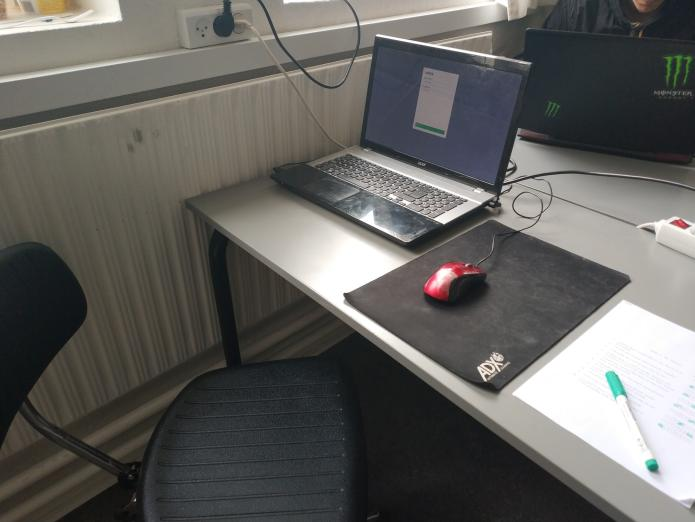
\includegraphics[width=0.75\linewidth]{InteraktionsDesign/Assets/Illustrationer/opstilling.jpg}
    \caption{The prototype is evaluated using this laptop setup, with the browser window in full screen}
    \label{fig:protypesetup}
\end{figure}

\begin{mdframed}[linewidth=0pt,backgroundcolor=lightgray!20,innertopmargin = 0.5cm,innerbottommargin = 0.5cm]
    \begin{enumerate}
        \item Firstly, the subjects are given a small introduction to the prototype. The subject also signs a form informing the subject of the intended use of the data, and their right to stop the evaluation at any time. The subject is sitting on a chair and using the setup seen in figure \ref{fig:protypesetup}.
        \item The subject now take a look on the log-in page of the prototype, and is then asked what they are looking at.
        \item The subject is now provided with the user name "test" and the password "123123", and is asked to log in.
        \item The subject is now asked to navigate the prototype, and find two endpoints:
        \begin{enumerate}
            \item The first navigation task is to send post a post to the forum called "Hacking" [Accessed via figure \ref{fig:prototype4}].
            \item The second navigation task is to find the post named "Facebook hacked last night!", and post a reply [Accessed via figure \ref{fig:prototype7}].
        \end{enumerate}
        \item After the subject has completed the navigation tasks, then he/she is asked about the general impression of the prototype.
        \item Lastly for the "think aloud" test, three additional questions are asked:
        \begin{enumerate}
            \item How clearly was the message of this being a secure platform conveyed?
            \item How could it be more clear?
            \item What will make you change to a more secure messaging platform? (From the main one the subject is using).
        \end{enumerate}
        \item The subject is now handed the SUS questionnaire.
        \item The evaluation ends after asking the subject about how he/she felt the evaluation was handled.
    \end{enumerate}
\end{mdframed}

\subsubsection{Problems}
During the think aloud test it was found that if we answered too many small questions the test could turn into a conversation. Therefore, ones experiment must have a well defined rule set such that the people running the experiment do not disturb the test themselves.\newline
Regarding the SUS some test subjects were confused as to whether they had to answer the survey based on the prototype presented to them or if they had to imagine how the "finished" product would rate on the different scales. This issue made it evident that the individual parts of the experiment need to be thoroughly explained, even when it seems straightforward.

\subsection{Results}
The user evaluation test was executed with a small sample size of 8 participants, they where also subject to the same procedure as described in section \ref{procedure}.

\subsubsection{Think aloud test results}
Common observations from the think aloud test. The full raw data is available in appendix \ref{appendix:thinkaloud}.
\begin{enumerate}
    \item Some participants felt the splash screen did not sufficiently explain the security concept. This refers to both the technical details but also the concept itself. 
    \item At least one participant thought the use of clip art on the splash screen lacked seriousness.
    \item One participant specifically noted, that a graphical explanation of the concept was nice, in contrast to a lot of text.
    \item Every participant thought one thing or another was somewhat unclear or misleading.
    \item Most of the participants thought the prototype was simple in design without much clutter.
    \item Several participants noticed the lack of a "forgot password" option and a "create account" option
    \item No participants were able to guess, that the product could utilise their own social media as part of the security concept.
    \item Some participants noticed that the log-in page gave no hints as to which product they were about to log in to. 
\end{enumerate}

\subsubsection{SUS test results}
Full raw data from the SUS test, can be found in appendix \ref{appendix:susvalues}. The data is also represented in a histogram as shown in Figure \ref{fig:histogram}. The histogram was made with a bin size of 5 and the data has a mean of 79.4 and a standard deviation of 4.49.

\begin{figure}[H]
    \centering
    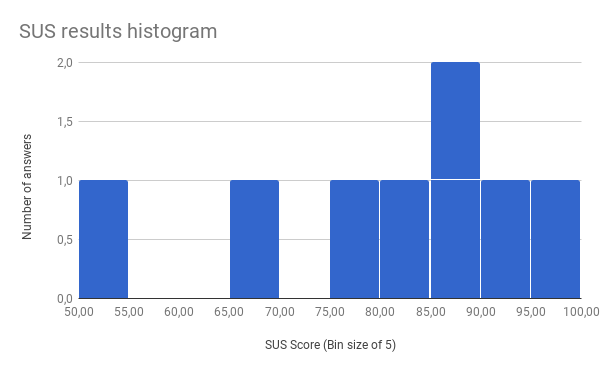
\includegraphics[width=0.75\linewidth]{InteraktionsDesign/Assets/Resultater/histogram_new.png}
    \caption{SUS test results visualised in a histogram with values:
        \mu  = 79.4  \newline SD = 4.49}
    \label{fig:histogram}
\end{figure}

\subsection{Discussion}
If we were to consider the SUS results as a standalone usability measurement, with a score of 68 being the threshold for good usability, then six out of eight test subjects deemed the usability good. However, since the SUS cannot be considered independently and the sample size is quite small, the overall usability might be somewhat lower. This is due to the fact that most of the test subjects thought some elements were lacking in explanation or downright confusing. One participant in particular was surprised that "Send post" referred to making a post on a forum. The participant thought that "Send post" was referring to sending a message to someone in particular. Steps should be taken to prevent such confusion. 
\newline
Another issue that surfaced during the experiment was the subject's understanding of the system's security concept. The splash screen presentation of the concept resulted in a number of problems. First off, at least one participant clicked right past the screen. This allowed for no information to be passed on to the user. Another user found the graphical representation of the concept to be childish, preferring text instead. However, another participant thought that the graphical representation of the concept was really good because this person would not have wanted to read a wall of text. From this it is clear that both types of users exist and they prefer differing communication styles. One might envision a splash screen that asks the user to chose a type of explanation. This is further supported be the fact that two test subjects had the opposite problems. One of these did not understand the splash screen because the subject could not decide how to interpret the images presented and therefore had difficulty understanding the concept. The other user was convinced that the images were to be interpreted in a very particular way. However, this subject then immediately started questioning the validity of the method, despite actual technical explanation being nowhere to be found. Obviously both users would benefit greatly from a longer written explanation. Again one might need to implement two different explanations, one in great technical detail and one in conceptual details. 
Expanding on this the seventh qualitative result further cements that the concept was too poorly explained. Given the fact that the product's most important feature is a specific kind of security that should provide an extensive anonymization capability, it is a must that this is conveyed properly. Furthermore, the understanding of this concept would also be important in using the finalised product since that version would include the option to use anonymous social media accounts as well as one's private account.